%hello document


\documentclass[11pt]{article}
\usepackage[top=2.54cm, bottom=2.54cm,left=1.27cm,right=1.27cm]{geometry}
\usepackage{graphicx} 
\usepackage{cite}
\usepackage{setspace}
\usepackage{listings}

\begin{document}

\title{Project Report for CS296 \\ Cheetah Simulation \\ Group 17}
\author{Naveen Sagar\\120050026 ,
 \texttt{120050026@cse.iitb.ac.in} \\
\and
Aditya Kumar Akash\\120050046 , \texttt{adityaakash@cse.iitb.ac.in} \\ 
\and
Prateek Chandan\\120050042 , \texttt{prateekchandan@cse.iitb.ac.in} \\
}
\date{\today}
\maketitle 
\newpage

\section{Indroduction}
This document gives details of the Project report for the course CS296 Software Systems Laboratory, taken by Prof Parag Chaudhary\cite{sir}. 
It contains The details of the new cheetah simulation.Cheetah is the fastest running animal on the planet.In out Box2D simulation project we have tried to model the simulation of cheetah's body , its balancing along with it's basic motion like walk and jump \\
\section{The Aniamtion}

\subsection{Model submitted in abstract}
The model submitted in the project proposal was : \\
Each legs has three moving parts connected to a hinge which is shown in the diagram. They can rotate and give motion to the model. Also the rib , tail and the neck of the model is made of small polygons which can swing and maitain the body of the cheetah.

\begin{figure}[!ht]
	\centering
		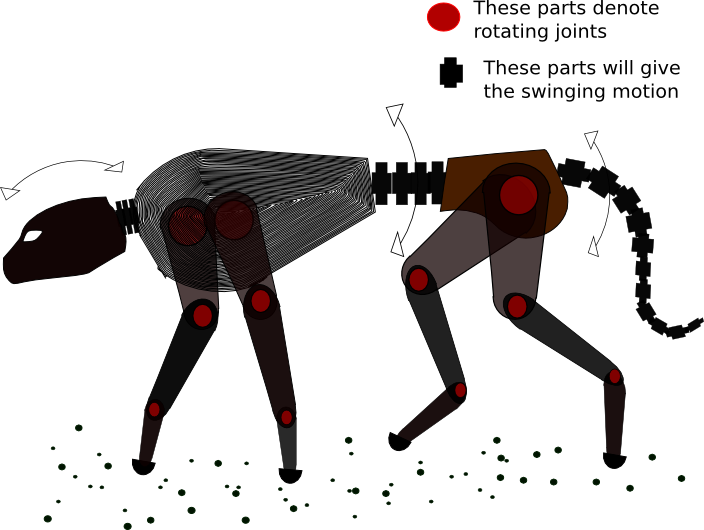
\includegraphics[scale=0.6]{drawing.png}
		\caption{The model submitted in abstract}
\end{figure}
\subsection{Final Box2d Model of the Cheetah}
The model submitted in the project proposal was : \\
Each legs has three moving parts connected to a hinge which is shown in the diagram. They can rotate and give motion to the model. Also the rib , tail and the neck of the model is made of small polygons which can swing and maitain the body of the cheetah.

\begin{figure}[!ht]
	\centering
		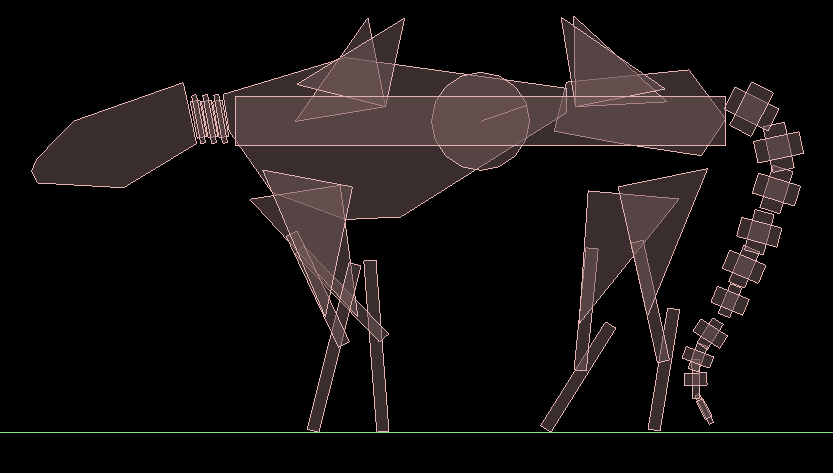
\includegraphics[scale=0.4]{final.png}
		\caption{The completed model in Box2D}
\end{figure}
\subsection{Deviation from the design}
\paragraph{Removals}
The part which is missed in the final design in the rib of the cheetah. The main reason to remove it was the balancing problem of the cheetah. As due to the changed and different body parts , a firm center part was required
\paragraph{Additions}
Wee added the muscles to the leg of the cheetah making the balancing of the cheetah to be more realistic and also we added Theo Jansen\cite{jansen} Walking mechanism for Cheetah which is a wheel based walking mechanism
\section{Physics behind the simulation and details of the mechanism used}
This section contains information about the different parts of cheetas body which is used in the animation
\begin{enumerate}
	  \item Walking Mechanism
	  \item The legs and Muscles
   	 \item The Tail
     \item Neck and Head
     \item Main body
\end{enumerate}
\subsection{Walking Mechanism}
The Walking Mechanism of cheetah is based on Theo Jansesn\cite{jansen} walking mechanism
\paragraph{Theo Jansen linkage}
It is a “crank-based” where the circular movement of
one point in the linkage translates to movement elsewhere in the linkage; this means the
circularly moving part of the li
nkage can be attached to a crank so that the motion of the
mechanism is easily driven allowing easy locomotion

\paragraph{}
\begin{figure}[!ht]
    \centering
        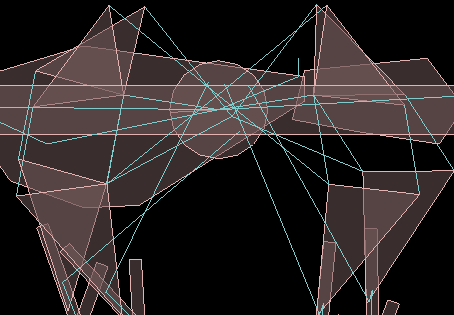
\includegraphics[scale=0.6]{jansen.png}
        \caption{The image showing Walking Mechanism}
\end{figure}


\subsection{The legs and Muscles}
\paragraph{Description of Leg}
There are 4 legs in total of the cheetah two in the front while two in the back. Each of the leg consists of two bony parts joined by the revolute joints with constraint in  the angle of rotation so as to maintain the shape of the leg\\
These legs are then joined by the theo jansen walking mechanism
\paragraph{Distance Joints as Muscles}
The walking mechanism is joined by distance joint which acts as springs which act as shock absorber for cheetah. It also helps in balancing of the body and legs after few deformations

\paragraph{}
\begin{figure}[!ht]
    \centering
        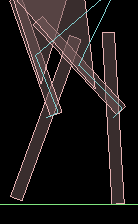
\includegraphics[scale=0.8]{joint.png}
        \caption{The image showing Distance joints as muscles}
\end{figure}

\subsection{The Tail}
\paragraph{} 
This part is cheetah's tail which consists of multiple small blocks joined together with revolute joints.The revolute joint in the tail is constrained with the the angle constaints . Total sum of constraint in the allows it to move totally while maintaining its initial shape. Since tail is the highly important in maintaining the body balance its weight is accurately set so that it gives proper motion to body
\newline
Each of the block itself is made of two rectangular blocks joined together


Due to the tail the angular mometum of the cheetah's body is balanced
\begin{figure}[!ht]
    \centering
        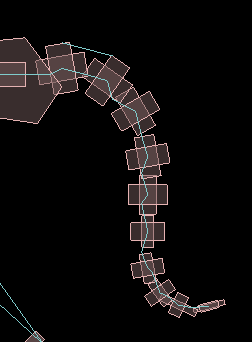
\includegraphics[scale=0.6]{tail.png}
        \caption{The image of tail consisting of multiple joints}
\end{figure}
\subsection{Head and the Neck}
\paragraph{} 
The head of the cheetah is a normal body mady of a convex polygon.While the neck is far more interesting. Thr neck consists of three blockes joined and packed closely with a revolute joint. This helps in the swingning motion of the neck of the cheetah.
\\
\begin{figure}[!ht]
    \centering
        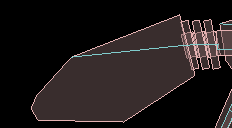
\includegraphics[scale=0.8]{head.png}
        \caption{The neck and head of cheetah}
\end{figure}
\subsection{Main body of cheetah}
\paragraph{} 
The main body of cheetah consists of a wide rectangular box to which all other parts of cheetah is joined. It acts a support for the whole body and helps in controlling the mwalking and jumping mechanism of cheetah.

The walking mechanism is at the center of this body and it controls whole of the walking of the cheetah

\section{What makes the Simulation Interesting}

The cheetah is the fastest land animal, achieving a top speed of about 70 mph (113 kph)\cite{facts} This is the main motivation toward taking up of this project. But owing the the restrictions of Box2D we tried to stimulate some of the parts of Cheetah's body and balancing and other details. Making a prototype of Living Organism which is the most complex machines makes our simulation interesting\\

While running the simulation you can see the swift swinging motion of tail, the motion of the head. Make the cheetah jum high and then land it to the ground. You can see the detailing of the landing and balancing. Such things also make the simulation interesting
\section{Profiling report of the code }
\paragraph{}
Using the profiling technique used in Lab09 we profiled the simulation of cheetah to find out the results
 
 \emph{We have used perf profiler to make the profile data.}\\
 \emph{No of iteration for data : 10000}

\subsection{Call Graphs}
A call graph is a directed graph that represents calling relationships between subroutines in a computer program.
Specifically, each node represents a procedure and each edge indicates that procedure f calls procedure g.\\

\textbf{Generation of call graph using perf and the gprof2dot.py} \\
\begin{lstlisting}
perf record -g -- ./mybins/cs296_17_exe
perf report > g17_release_prof.dat
perf script | python gprof2dot.py -f perf | dot -Tpng -o release.png
\end{lstlisting}

\begin{figure}[h!]
	\centering	
		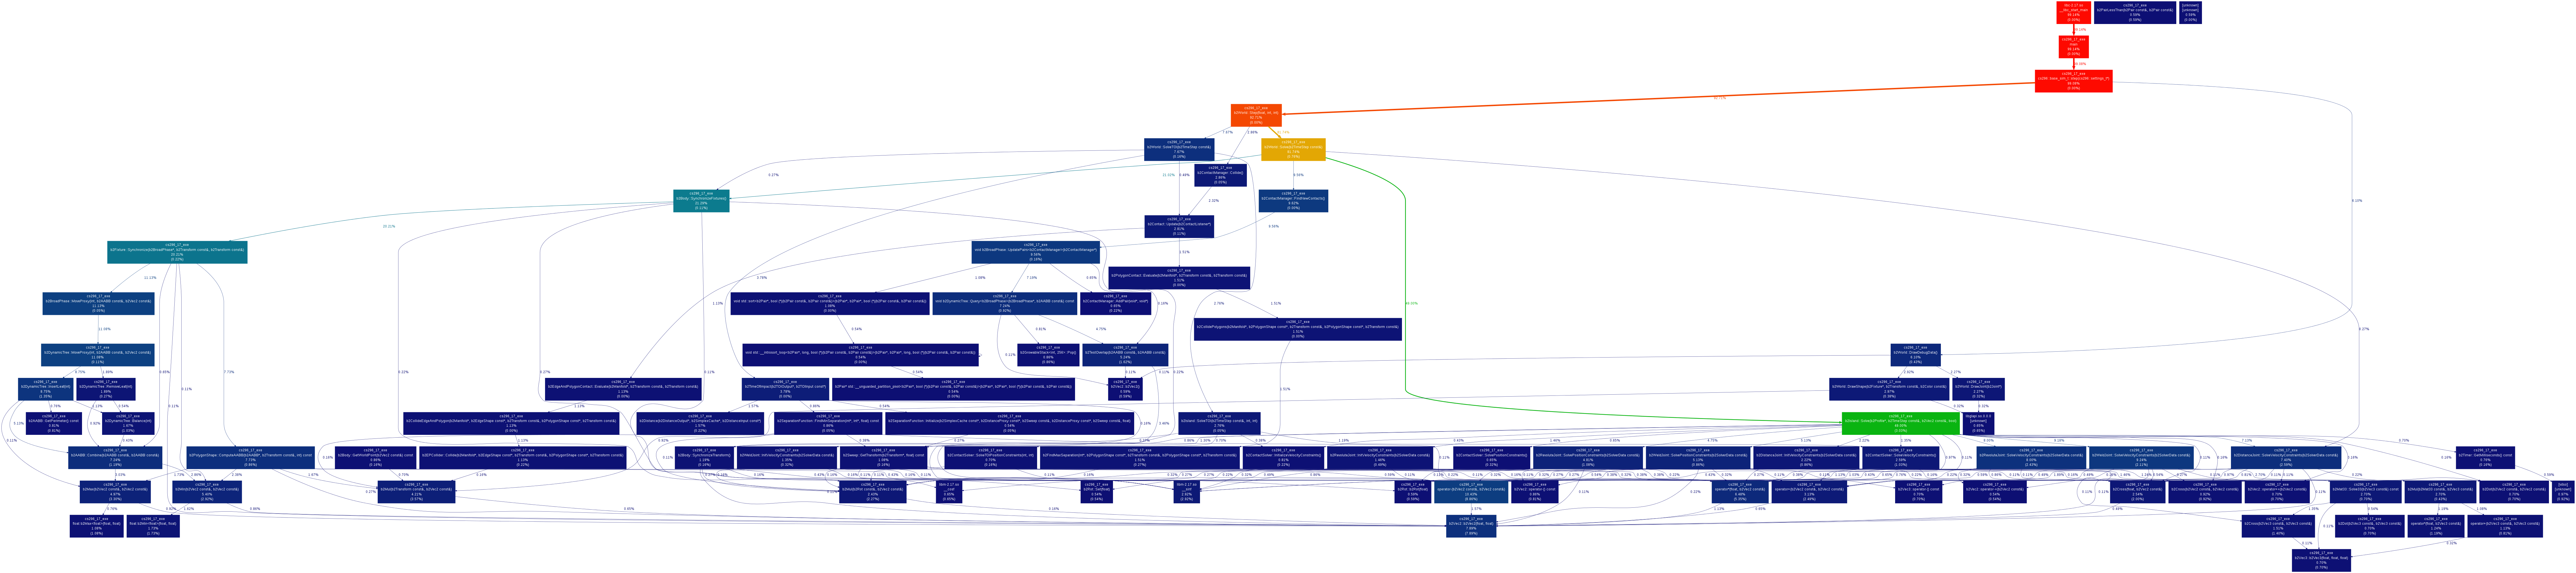
\includegraphics[width=1\textwidth]{debug.png}
		\caption{Debug Call Graph}
\end{figure}

\subsection*{Observation from Debug Call Graph}
List of Functions which consume most time in the call of their parents
\begin{enumerate}
    \item b2World::step() 92.00 \%
    \item b2World::solve() 49.00 \%
    \item b2RevoluteJoint::SolveVelocityConstraints() 8.00 \%
    \item b2DistanceJoint::SolveVelocityConstraints() 9.24 \%
    \item b2weldJoint::SolveVelocityConstraints() 9.24 \%
    \item b2Fixture::SynchronizeFixture() 21.29 \%
    \item b2Fixture::Synchronize() 20.00 \%
    \item b2BroadPhase::MoveProxy() 11.00 \%
    \item b2BroadPhase::UpdatePairs(b2ConstactManager) 9.56 \%
    \item b2DynamicTree::querry() 7.24 \%
    
\end{enumerate}

\begin{figure}[h!]
	\centering
		
\includegraphics[width=1\textwidth]{release.png}
			\caption{Release Call Graphs}
\end{figure}

\subsection*{Observation from Release Call Graph}
List of Functions which consume most time
\begin{enumerate}
    \item b2RevoluteJoint::SolveVelocityConstraints() 4.76 \%
    \item b2DistanceJoint::SolveVelocityConstraints() 4.48 \%
    \item b2weldJoint::SolveVelocityConstraints() 3.92 \%
    \item solve() 5.20 \%
    \item b2Timer::GetMilliseconds() 3.86 \%
    \item b2DynamicTree::Querry() 6.74 \%
    \item b2Fixture::synchronize() 0.80 \%
\end{enumerate}

\subsection{Analysis of above Call Graphs}
\textbf{General Analysis} :\\
\textbf{Debug Mode} :\\
As we can see from the callgraph and the most time consuming functions , debug mode calls much more functions as compared to the call graph of release mode.
Most of the time is consumed by the calculating functions which are solve , solveVelocityContraints etc 
consumes most of the time as compared to the Drawshape funstion and drawDebug function\\
\textbf{Release Mode} :\\
As opposed to the times in Debug mode , The Drawshape function take the most time in the running of the function while the solving function functions like
solveVelocityContraints and solve function took time much lesser than that in debug mode. also the system library used for calculation took very less
time \\
\textbf{Special Analysis w.r.t The Project Code } : \\
Clearly we can see that the functions related to synchronizing fixtures and collision detection such as - \emph{SynchronizeFixture() and FindNew Manager}
take more as compared to profiling done in earlier labs.\\
Also the Functions related to BroadPhase which manages the proxies ( - representing the AABB's in broadPhase collision algorithm ) 
and the creation and deletion of records w.r.t the overlap of proxies such as
\emph{MoveProxy(), UpdatePair(), InsertLeaf(), Querry()} take much time as compared to previous profiling. \\
Moreover the functions ( SolveVelocityConstraints() )  related to solving the constraints equations for the joints - \emph{Revolute, Weld and Distance} take more time in comparision.


\subsection{Inference from the above Analysis}

\textbf{General Inference}
We can clearly see that the Debug mode is taking more time for all the functions in comparision to the release mode which does the optimization.\\
The function \emph{solveVelocityConstraint()} and \emph{solve()} takes more time in both the modes.
The step function is taking a lot of time in the debug mode as it is the function which is called again and again. \\
The \emph{DrawShape()} takes significant amount of time as this function is called each time the \emph{step()} function is called.
This function is responsible for updating the position of the various objects on the frame after the solving of all velocity and position 
constraint equation is solved. So it is natural for this function to take more time. \\
The library \_mcount takes more time in the debug mode but negligible amount in release mode and hence no need to optimize thus library.\\

\textbf{Special Inference wrt Project Objects}
We can clearly see that the program spends a lot of time in handling the different fixtures.
The functions which are responsible for obtaining the overlap of fixture proxies - ( the AABB's representation ) and storage
of these in a dynamic tree consumes lot of time. 
The behaviour is justified since we have a lot of fixtures which are overlapping and many of them are using collision filtering
using \emph{filter.groupIndex} . Thus the box2d engine has to spend a lot time to decide which of them to collide and which not.
Moreover we have 2 bodies - \textbf{tail, neck} which is made of lot of smaller bodies joined together and spaced very close to each other .
Thus the contact equations are to be solved more often for the fixtures of these bodies.
Also due to lot of smaller bodies connected to form larger bodies we get a lot of joints of all kinds. Hence the constaint equations for 
these joints are solved more often thus explaining the cause that SolverVelocityConstraints() of these joints take a large time.

\subsection{Optimizations Required}
Refering to the above Inference we see that we would have to decrease the number of pieces that makes the tails and the neck. 
But such a process would result in destroying the flexible movement of the tail and neck and thus changing the expected behaviour.
So we changed the spacing and arragement of the object in neck . Also for tail the fact that we could initialize the same body with
different fixtures was used to decrease the number of bodies actually making the tail .\\
For different fixtures that were using the groupIndex to do collision filtering we tried to expolit the fact we used for tail.
But the mass distribution which maitained the overall balance of the cheetah on its legs and helped the crank system to make it move smoothly
got unbalanced cauising some unexplained behaviour . Hence we had to compromise in this optimization by designing the bodies so that balance 
is also maintained and the overlapping parts overlap as less as aloowed so that the movement is smooth. 

\section{Analysis Report for the plots my Matplotlib}
This section contains the Reports , Obsevations and Inference from the timing diagram which are obtained from the data and the 
Plots generated using matplotlib of the project simulation.\\
No of Iteration for which the 	the iteration was run for 1 to 500 and 50 rerun for each iteration
\subsection{Observation from Plot1}
The following inference were drawn from the Plot1 diagram which was Plot of Average Step time  and Average loop time:
\begin{enumerate}
    \item The Average loop time is greater than the Average Step Time but is almost equal
    \item The average time for the decreases as the no of iteration increases
\end{enumerate}
\textbf{Explanation:}
Since for the first few iterations the world is being set and all the objects in a state of movement to get settled to there stable state
and also the no of of collisions taking place are too high, the time taken by the Loop in fisrt few Interation are High.
But as he loop progresses the animation gradually takes place without much calcualtion or updates and the updates are very few so the time for 
the further loops decreases. Due to this the average time for more iterations decreases as compared o lesser no of Iterations\\

Since the step time is the of all times taken by the loop while the loop time is the total time taken by the loop in addition to the Time 
taken by system processes so the loop time is slightly greater than the step time. And when the same was generated while the sytem was overloaded 
with programs, This gap was still greater.
\begin{figure}[!ht]
	\centering
	\caption{Plot1}
		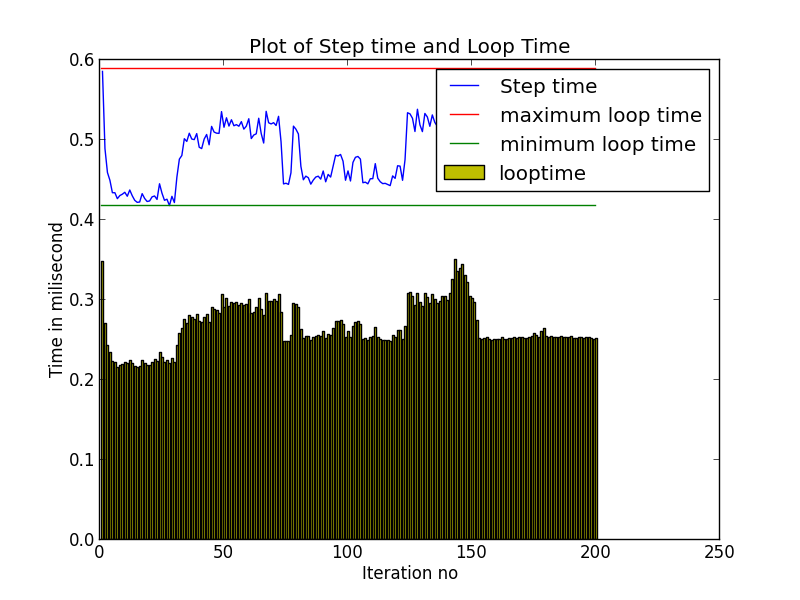
\includegraphics[scale=0.5]{../plots/g17_plot01.png}
\end{figure}
\subsection{Observation from Plot2}
The following inference were drawn from the Plot2 diagram which was Plot of Step time , Collision time , Velocity update time , Position update time
and sum of last 3 averaged:
\begin{enumerate}
    \item The step time is greater than the sum of Collision time , velocity update time and position update time
    \item All of these times decreases as the no of iteration increases
\end{enumerate}
\textbf{Explanation:}
The step time is the time taken by the loop which is running the Animation. But the other three times are exactly what they are meant to be.
But since the step time is the time taken by all of the things within a loop , So there are other processes which will also be called within the for loop 
and they will take time increasing the step tme\\

The explnation for initial times to be greater as the explanation in of Plot1
\begin{figure}[!ht]
	\centering
	\caption{Plot2}
		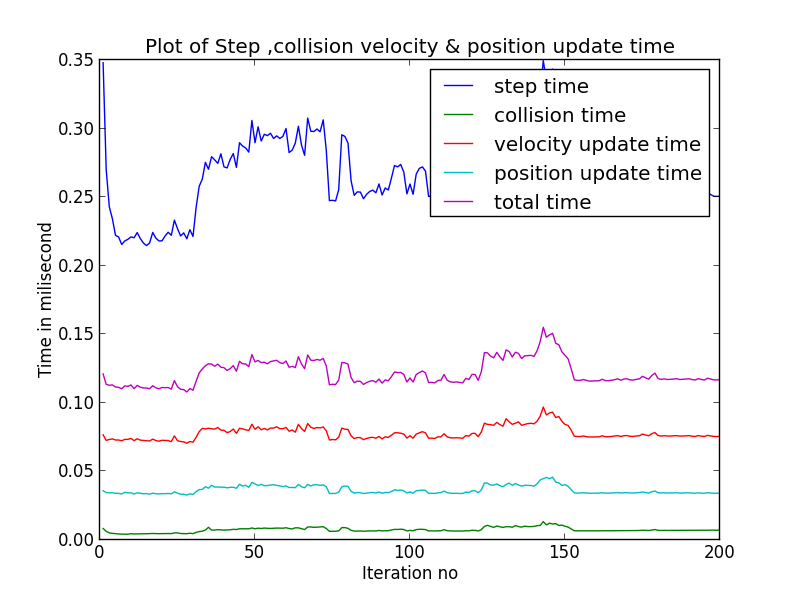
\includegraphics[scale=0.5]{../plots/g17_plot02.png}
\end{figure}
\subsection{Observation from Plot3}
The plot3 was the plot of averaged step time along with error bars calculated with standard deviation\\

It is observed that the error bars for the average stem time for lower no of iterations was too high as compared to the error
 bar for higher no of iterations \\
 
This might be because of the reasons explained in Plot1. Since the setting of world can take place differently for only one iteration because of 
setting up of worlds and setting up of initial position of objects so the error bar is too high. But when the no of iteration is high, This total 
time sums up to almost be equal. So the standard deviation is low making the error bar to be small. 
\begin{figure}[!ht]
	\centering
	\caption{Plot3}
		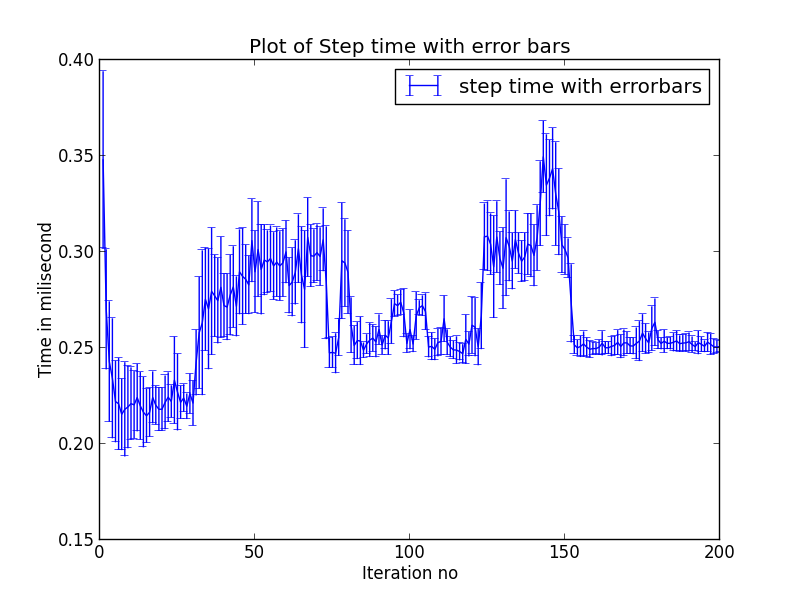
\includegraphics[scale=0.5]{../plots/g17_plot03.png}
\end{figure}
\subsection{Observation from Plot4}
When the step time gets averaged up it keeps fluctuating around the the average value which comes out to be 
0.94 second and the rest of the times are around it.\\

But there is an Outlier time which denotes the time at the start of the loop. Since  At the beggining the times are higher so they 
contribute for a frequency of a higher time
\begin{figure}[!ht]
	\centering
	\caption{Plot4}
		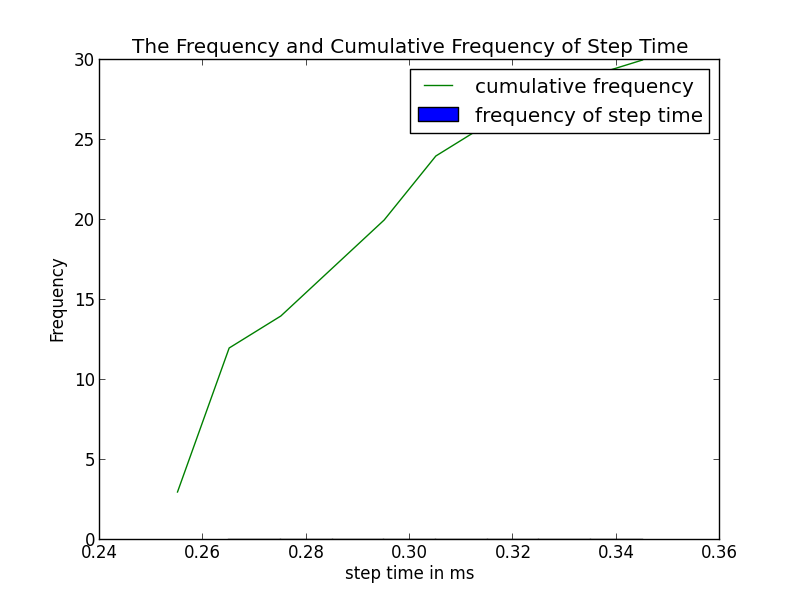
\includegraphics[scale=0.5]{../plots/g17_plot04.png}
\end{figure}
\subsection{Observation from Plot5}
Plot 5 was the plot for the best fit line for the step time averaged over all data and step time averaged over some random data
\begin{enumerate}
    \item The points for the averaged time of all data and random data are almost equal 
    \item The best fit line comes to be almost same for both of them
\end{enumerate}
\textbf{Explanation:}
	Since the time for a particular iteration is almost the same so it doesnt matter much if the points are averaged over all data or 
the  points are averaged over only few random data. Due to this the points comes to be nearly the same and also the best fit line is nearly 
the same
\begin{figure}[!ht]
	\centering
	\caption{Plot5}
		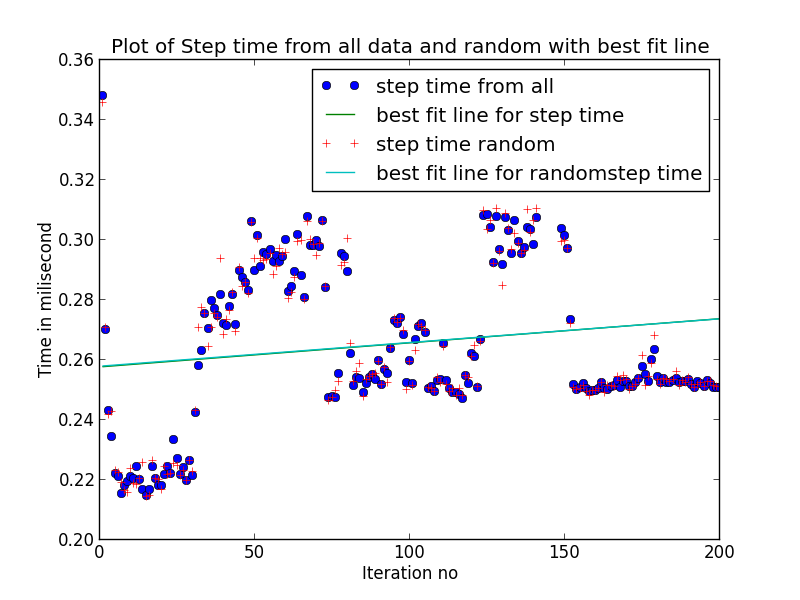
\includegraphics[scale=0.5]{../plots/g17_plot05.png}
\end{figure}
\section{Conclusion}
\paragraph{Project}
The cheetah simulation along with finishing of the project was very intersting and of great learnig experience. We learnt various aspects of complex machine simulation , different walking mechanism used by cheetah , Implementation in box2D with a simpler walking mechanism , simulating body parts like tail and neck of the cheetah and other things. The amount of learning experience from this project was too great.
\paragraph{CS296 course}
This CS296 was overall a great learning ecperience of Box2D and also other software development techniques. In the CS296 course as a whole we learnt a lot and we are very thankful to the instructor Prof Parag Chaudhary\cite{sir}. The software development techniques learnt and the other very usefull softwares learnt has increased \emph{geekiness} in us. And we will continue our the Coding aspect followed up from this course.

\bibliographystyle{plain}

\bibliography{cs296_report_17}

\end{document}

